% gepisat-3_stage1.tex
%
% written by Tyler W. Davis
% Imperial College London
%
% 2014-10-29 -- created
% 2014-10-29 -- last updated
%
% ------------
% description:
% ------------
% This TEX file contains Part 3 modeling Stage 1 for the GePiSaT model documentation.
%
% ----------
% changelog:
% ----------
% 01. modularized chapter [14.10.29]
% 02. newline for each sentence [14.10.29]
% --> simpler for Git version control
%
%% \\\\\\\\\\\\\\\\\\\\\\\\\\\\\\\\\\\\\\\\\\\\\\\\\\\\\\\\\\\\\\\\\\\\\\\\ %%
%% PART 3.2 -- STAGE 1
%% //////////////////////////////////////////////////////////////////////// %%
\section{Stage 1: Flux Partitioning}
\label{sec:mst1}
The first step in this modeling process is the empirical partitioning of high temporal resolution CO$_{2}$ flux data into quantities of gross primary production (GPP) and ecosystem respiration (R$_{\mathrm{e}}$).  
The partitioning is based on pairing the CO$_{2}$ flux data with in situ photosynthetic photon flux density (PPFD) measurements.

%% \\\\\\\\\\\\\\\\\\\\\\\\\\\\\\\\\\\\\\\\\\\\\\\\\\\\\\\\\\\\\\\\\\\\\\\\ %%
%% PART 3.2.1 -- STAGE 1: DATA
%% //////////////////////////////////////////////////////////////////////// %%
\subsection{Data}
\label{sec:mst1data}
High temporal resolution CO$_2$ flux data is acquired by means outlined in \S \ref{sec:gepfluxd}.  
The half-hourly synthesis data is processed to remove all non-observational and low quality data.  
In the current model, only observations of NEE and PPFD are retained from the original files.

%% \\\\\\\\\\\\\\\\\\\\\\\\\\\\\\\\\\\\\\\\\\\\\\\\\\\\\\\\\\\\\\\\\\\\\\\\ %%
%% PART 3.2.2 -- STAGE 1: METHODOLOGY
%% //////////////////////////////////////////////////////////////////////// %%
\subsection{Methodology}
\label{sec:mst1meth}
The methodology for flux partitioning is based, in part, on Ruimy et al., 1995 \parencite{ruimy95}.  
The derivation of the empirical partitioning equation begins with the fundamental definition of net ecosystem exchange (NEE)\parencite{lovett06}:
%% ------------------------------------------------------------------------ %%
%% eq:nee | Net ecosystem exchange
%% ------------------------------------------------------------------------ %%
\nomenclature{$\text{NEE}$}{Net ecosystem exchange [$\mu$mol CO$_{2}\cdot$m$^{-2}\cdot$s$^{-1}$]}%
\nomenclature{$\text{R}_{\text{e}}$}{Ecosystem respiration [$\mu$mol CO$_{2}\cdot$m$^{-2}\cdot$s$^{-1}$]}%
\nomenclature{$\text{GPP}$}{Gross primary production [$\mu$mol CO$_{2}\cdot$m$^{-2}\cdot$s$^{-1}$]}%
\begin{equation}
\label{eq:nee}
    \text{NEE} = \text{R}_{\text{e}} - \text{GPP}
\end{equation}

\noindent The convention presented in equation \ref{eq:nee} indicates that positive CO$_{2}$ exchange occurs in the form of ecosystem respiration (i.e., adding CO$_{2}$ into the atmosphere) and negative exchange occurs during photosynthesis (i.e., atmospheric carbon sequestration into plant leaves). 
There are several models that combine leaf photosynthesis (e.g., GPP) and radiation transfer (e.g., PPFD) through a vegetated canopy.  
In \parencite{ruimy95}, the response curve of leaves to radiative energy is assumed to follow one of two models described below (rearranged for consistency with the sign convention presented in equation \ref{eq:nee}).  
Equation \ref{eq:modell} represents the ``linear'' response model and equation \ref{eq:modelh} represents the ``rectangular hyperbola'' response model.
%% ------------------------------------------------------------------------ %%
%% eq:modell | GPP partitioning (Ruimy's linear model)
%% ------------------------------------------------------------------------ %%
\nomenclature{$F$}{CO$_{2}$ exchange rate [$\mu$mol CO$_{2}\cdot$m$^{-2}\cdot$s$^{-1}$]}%
\nomenclature{$R$}{$F\left(Q=0\right)$  [$\mu$mol CO$_{2}\cdot$m$^{-2}\cdot$s$^{-1}$]}%
\nomenclature{$\alpha$}{Apparent quantum yield [unitless]}%
\nomenclature{$Q$}{Quantum flux density [$\mu$mol$\cdot$m$^{-2}\cdot$s$^{-1}$]}%
\begin{equation}
\label{eq:modell}
    F = R - \alpha Q
\end{equation}

%% ------------------------------------------------------------------------ %%
%% eq:modelh | GPP partitioning (Ruimy's hyperbolic model)
%% ------------------------------------------------------------------------ %%
\nomenclature{$F_{\infty}$}{$F\left(Q_{sat}\right)$ [$\mu$mol CO$_{2}\cdot$m$^{-2}\cdot$s$^{-1}$]}
\begin{equation}
\label{eq:modelh}
    F = R - \frac{\alpha Q \cdot F_{\infty}}
          {\alpha Q + F_{\infty}}
\end{equation}

\noindent where $F$ is the CO$_2$ exchange rate, $R$ is the dark respiration rate, $\alpha$ is the apparent quantum yield (i.e., d$F$/d$Q$ at $Q=0$), $Q$ is the quantum flux density (e.g., PPFD), and $F_{\infty}$ is the CO$_{2}$ exchange rate at saturating quantum yield. 

By combining equations \ref{eq:modell} and \ref{eq:modelh} with equation \ref{eq:nee}, GPP partitioning can be obtained by setting $\text{NEE} = F$ and $\text{R}_{\text{e}} = R$. 
By making these substitutions into equations \ref{eq:modell} and \ref{eq:modelh}, the flux partitioning (i.e., equation \ref{eq:nee}) can be calculated in terms of measurable quantities (i.e., $F$ and $Q$) as shown in equations \ref{eq:linmod} and \ref{eq:hypmod}.
%% ------------------------------------------------------------------------ %%
%% eq:linmod | Linear model for Stage 1
%% ------------------------------------------------------------------------ %%
\nomenclature{$\text{PPFD}$}{Photosynthetic photon flux density [$\mu$mol$\cdot$m$^{-2}\cdot$s$^{-1}$]}
\begin{equation}
\label{eq:linmod}
    \text{NEE} = R - \alpha \cdot (\text{PPFD})
\end{equation}

%% ------------------------------------------------------------------------ %%
%% eq:hypmod | Hyperbolic model for Stage 1
%% ------------------------------------------------------------------------ %%
\begin{equation}
\label{eq:hypmod}
    \text{NEE} = \frac{a \cdot (\text{PPFD}) + b}{c \cdot (\text{PPFD}) + d}
\end{equation}

\noindent where:
%% ------------------------------------------------------------------------ %%
%% eq:shyp | Hyperbolic model definition of parameters
%% ------------------------------------------------------------------------ %%
\begin{subequations}
\label{eq:shyp}
\begin{align}
    a&= \alpha R - \alpha F_{\infty} \label{eq:shypa}\\
    b&= F_{\infty} R \label{eq:shypb}\\
    c&= \alpha \label{eq:shypc}\\
    d&= F_{\infty} \label{eq:shypd}
\end{align}
\end{subequations}

\noindent Note that the form of the rectangular hyperbola presented in equation \ref{eq:hypmod} has an x-axis asymptote defined by $a/c$ from equations \ref{eq:shypa} and \ref{eq:shypc}. 

In the linear model (i.e., equation \ref{eq:modell}), GPP partitioning can now be made by equation \ref{eq:gppl} and in the rectangular hyperbola model (i.e., equation \ref{eq:modelh}), GPP partitioning is made by equation \ref{eq:gpph}.
%% ------------------------------------------------------------------------ %%
%% eq:gppl | GPP partitioned (Ruimy's linear model)
%% ------------------------------------------------------------------------ %%
\begin{equation}
\label{eq:gppl}
    \text{GPP} = \alpha Q
\end{equation}

%% ------------------------------------------------------------------------ %%
%% eq:gpph | GPP partitioned (Ruimy's hyperbolic model)
%% ------------------------------------------------------------------------ %%
\begin{equation}
\label{eq:gpph}
     \text{GPP} = \frac{\alpha Q \cdot F_{\infty}}{\alpha Q + F_{\infty}}
\end{equation}

Figure \ref{fig:parti} presents example months of flux partitioning from four flux towers.  
In Figs. \ref{fig:parti} a and c, the trend between NEE and PPFD observations suits the hyperbolic model (i.e., equation \ref{eq:hypmod}), $R^{2}$ is 0.91 and 0.93, respectively. 
On the contrary, the trend presented in figure \ref{fig:parti} b can not be clearly distinguished as linear from hyperbolic as both models perform equally well ($R^{2}$ is 0.90 and 0.91 for the linear and hyperbolic fits, respectively). 
The high level of variability in figure \ref{fig:parti} d results in poor regression fitting and is therefore difficult to distinguish between hyperbolic and linear model fits ($R^{2}$ is $\approx$0.1 for both linear and hyperbolic model fits).

Now that the two partitioning models have been defined (i.e., equations \ref{eq:linmod} and \ref{eq:hypmod}), the next step is to begin the data processing.  
%% ------------------------------------------------------------------------ %%
%% fig:parti | Partitioning PPFD:NEE pairs
%% ------------------------------------------------------------------------ %%
\begin{figure}[h!]
    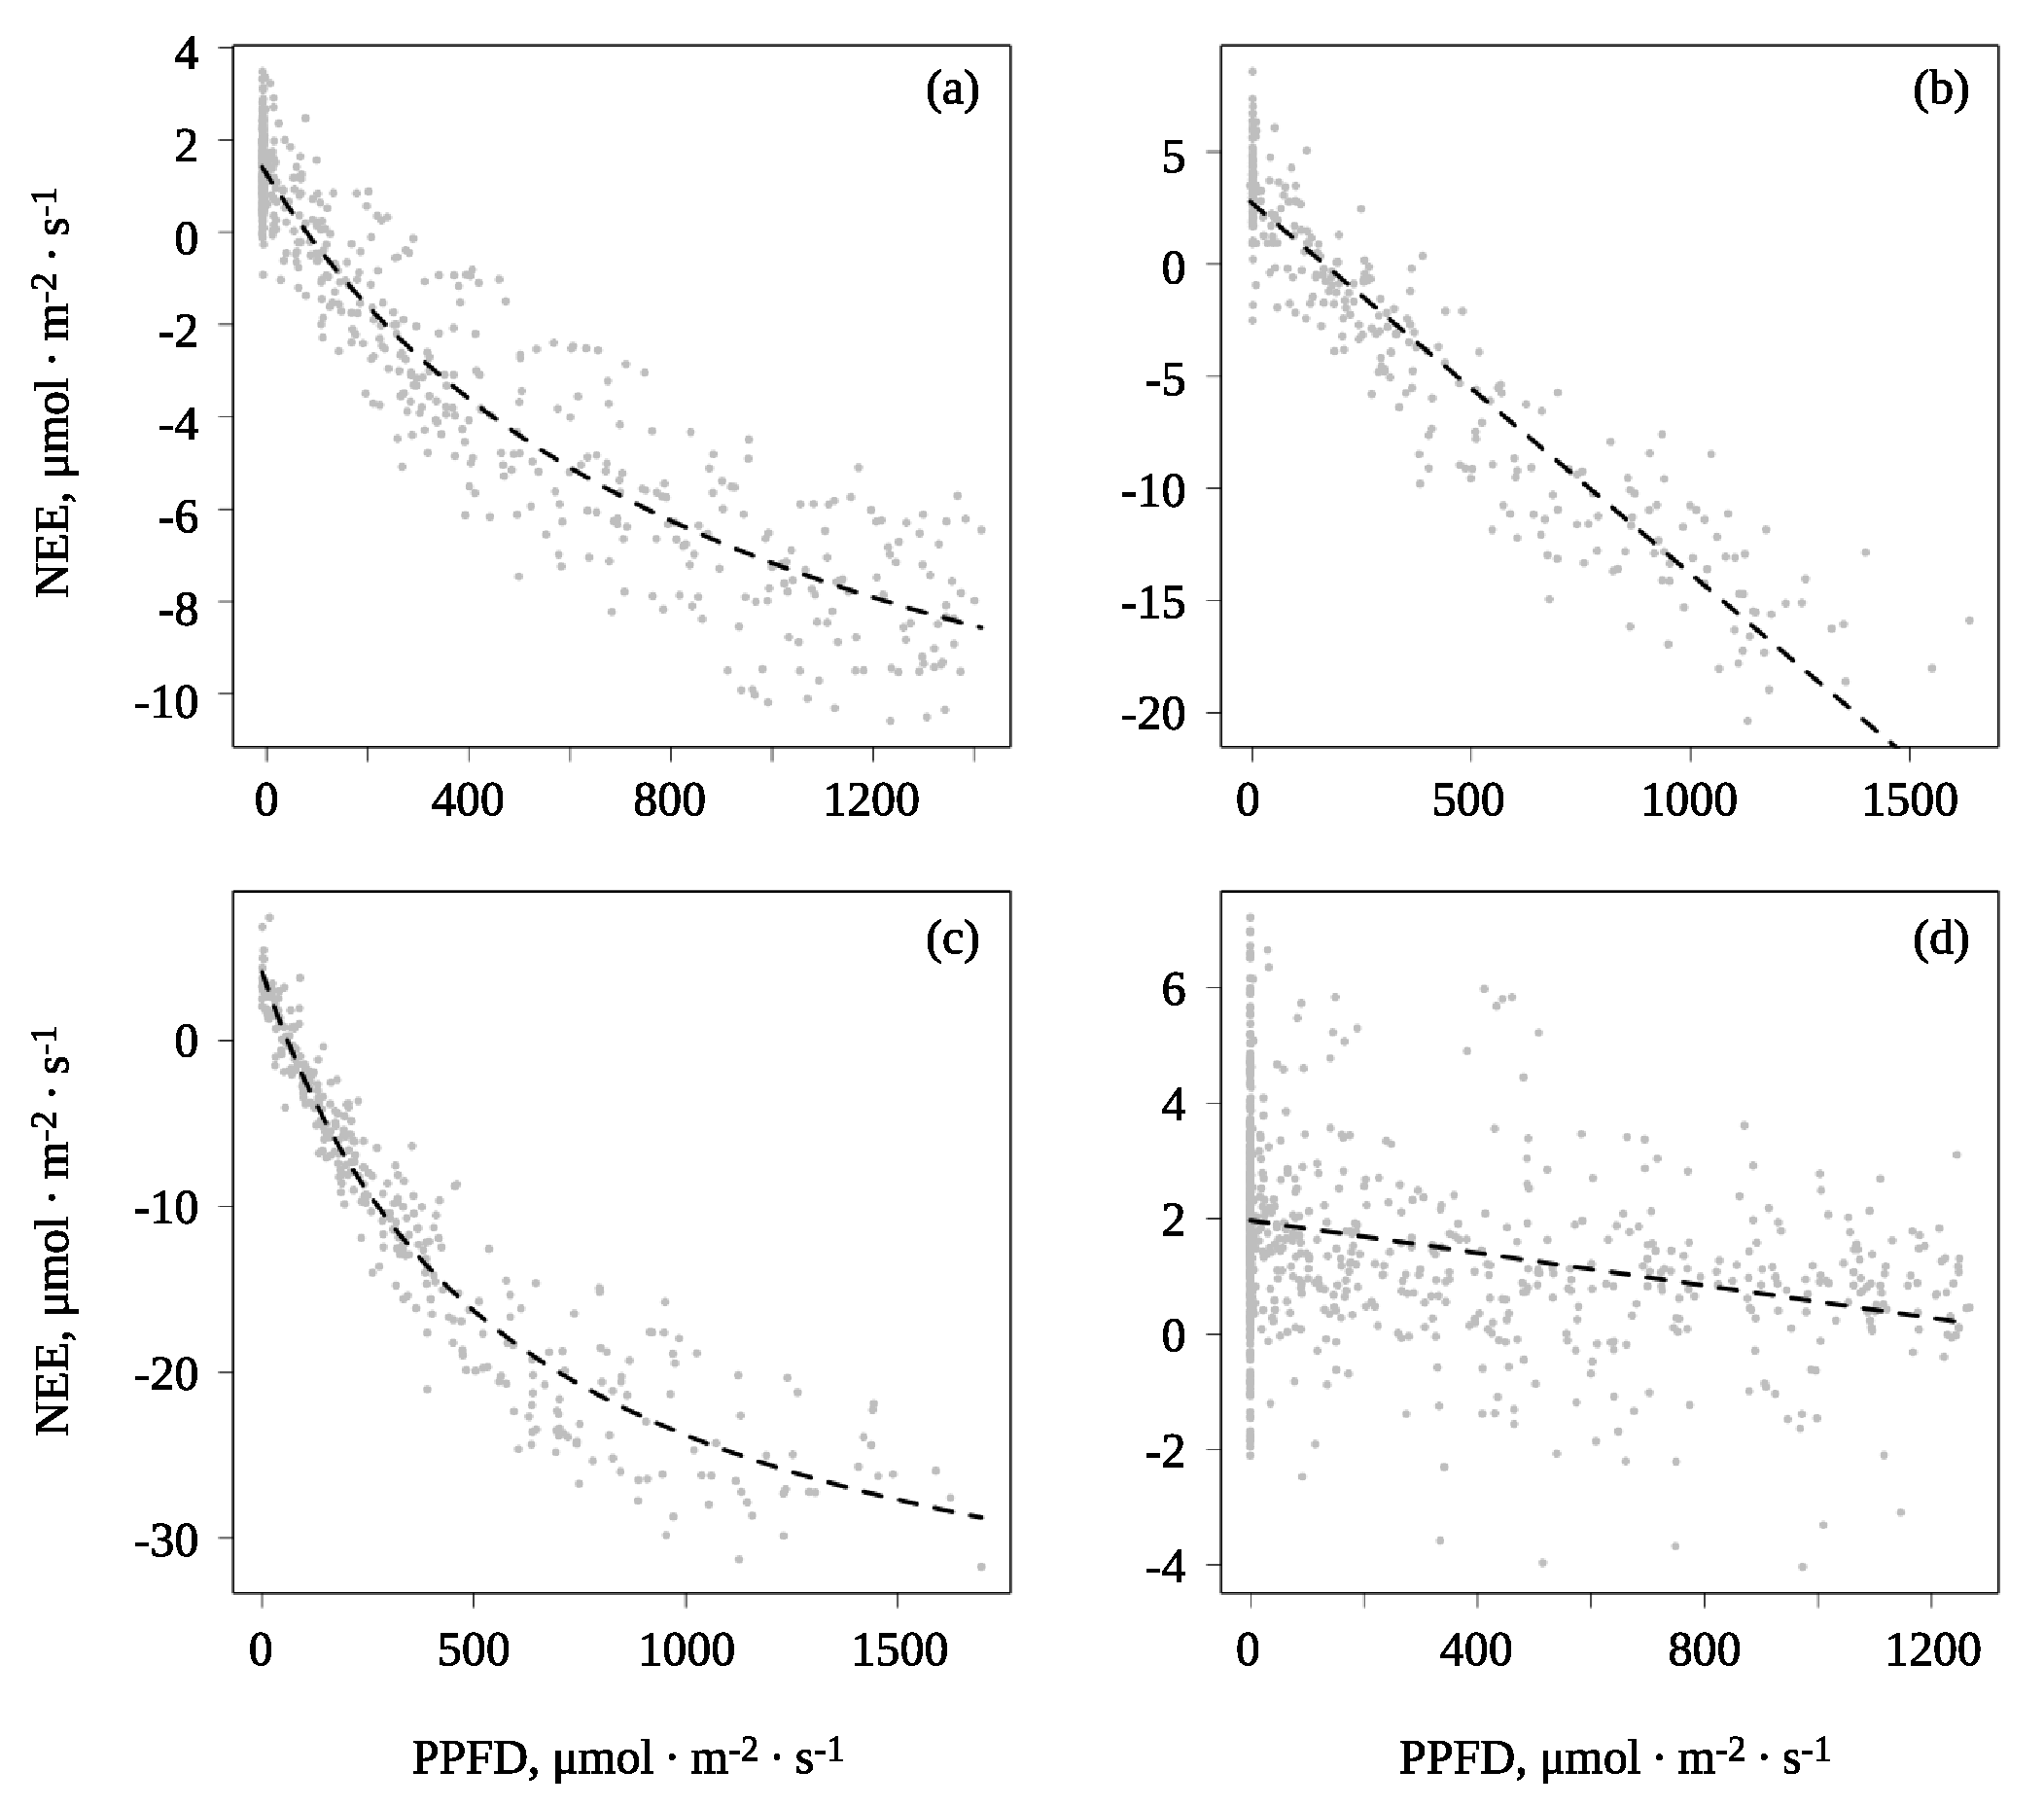
\includegraphics[width=\textwidth]{parti.eps}
    \caption{Flux partitioning of NEE and PPFD observations for stations (a) IL-
    Yat, Israel (Jan. 2002); (b) BE-Bra, Belgium (Aug. 2002); (c) DE-Hai, 
    Germany (Jul. 2002); (d) FR-Hes, France (Mar. 2002).  Data are fitted with 
    the rectangular hyperbola model in (a) and (c) and the linear model in (b) 
    and (d). }
    \label{fig:parti}
\end{figure}

%% \\\\\\\\\\\\\\\\\\\\\\\\\\\\\\\\\\\\\\\\\\\\\\\\\\\\\\\\\\\\\\\\\\\\\\\\ %%
%% PART 3.2.3 -- STAGE 1: ERROR PROPAGATION
%% //////////////////////////////////////////////////////////////////////// %%
\subsection{Error propagation}
\label{sec:mst1errprop}
During the flux partitioning of NEE and PPFD observations, the fitting parameters used to calculate GPP (i.e., Eq. \ref{eq:gppl} and Eq. \ref{eq:gpph}) are estimated.  
The parameter estimates include some uncertainty or associated error.  
To account for these errors in the calculation of GPP, a methodology of arithmetic error propagation is employed \parencite{caldwell14}.  
The general formula for the error propagation where $Y=f(A,B,C)$ is given as \parencite{ku66}:
%% ------------------------------------------------------------------------ %%
%% eq:errprop | Propagation of Error
%% ------------------------------------------------------------------------ %%
\begin{equation}
\label{eq:errprop}
	s_{y} = \sqrt{
		\left(\frac{\partial Y}{\partial A}\right)^{2} \cdot s_{a}^{2} +
		\left(\frac{\partial Y}{\partial B}\right)^{2} \cdot s_{b}^{2} +
		\left(\frac{\partial Y}{\partial C}\right)^{2} \cdot s_{c}^{2}
		}
\end{equation}

\noindent where:\\
\indent $s$ = standard deviation (i.e., error)\\

For the rectangular hyperbola formula for GPP (i.e., Eq. \ref{eq:gpph}), let $A = \alpha$, $B = F_{\infty}$, and $C = \text{PPFD}$ such that:
%% ------------------------------------------------------------------------ %%
%% eq:hpartial | Partial derivatives for error propagation:
%% ------------------------------------------------------------------------ %%
\begin{subequations}
\label{eq:hpartial}
\begin{align}
    \frac{\partial Y}{\partial A}&= \frac{F_{\infty} \cdot \text{PPFD} \cdot 
                                    \left( \alpha \cdot \text{PPFD} + F_{\infty} 
                                    \right) - \alpha \cdot F_{\infty} \cdot 
                                    \text{PPFD}^{2}}{\left(\alpha \cdot 
                                    \text{PPFD} + F_{\infty} \right)^{2}} 
                                    \label{eq:hparta}\\
    \frac{\partial Y}{\partial B}&= \frac{\alpha \cdot \text{PPFD} \cdot 
                                    \left( \alpha \cdot \text{PPFD} + F_{\infty} 
                                    \right) - \alpha \cdot F_{\infty} \cdot 
                                    \text{PPFD}}{\left(\alpha \cdot 
                                    \text{PPFD} + F_{\infty} \right)^{2}} 
                                    \label{eq:hpartb}\\
    \frac{\partial Y}{\partial C}&= \frac{\alpha \cdot F_{\infty} \cdot 
                                    \left( \alpha \cdot \text{PPFD} + F_{\infty} 
                                    \right) - \alpha^{2} \cdot F_{\infty} \cdot 
                                    \text{PPFD}}{\left(\alpha \cdot 
                                    \text{PPFD} + F_{\infty} \right)^{2}}  
                                    \label{eq:hpartc}
\end{align}
\end{subequations}

By substituting Eqs. \ref{eq:hparta}--\ref{eq:hpartc} into Eq. \ref{eq:errprop} and assigning the corresponding error values to $s_{a}$, $s_{b}$, and $s_{c}$ (note: the measurement of PPFD is assumed to be error-free, $s_{c} = 0$) the associated error for GPP can be calculated. 

In the more trivial case of the linear equation for GPP (i.e., Eq. \ref{eq:gppl}), the error propagation is directly proportional to the coefficient $alpha$ and its associated error.

%% \\\\\\\\\\\\\\\\\\\\\\\\\\\\\\\\\\\\\\\\\\\\\\\\\\\\\\\\\\\\\\\\\\\\\\\\ %%
%% PART 3.2.4 -- STAGE 1: DYNAMIC PARAMETERIZATION
%% //////////////////////////////////////////////////////////////////////// %%
\subsection{Dynamic parameterization}
\label{sec:mst1dyn}
The partitioning methods described in section \ref{sec:mst1meth} require fitting parameters to equations \ref{eq:linmod} (i.e., $\alpha$ and $R$) and \ref{eq:hypmod} (i.e., $F_{\infty}$, $\alpha$, and $R$). 
To perform the regression analysis, these parameters must first be given an initial condition or a guessed value.  
Linear regressions tend to be robust against initial conditions while hyperbolas can be sensitive to initial conditions, especially around y-axis asymptotes.  
One approach is to statically assign initial values to each parameter.  
However, to dynamically assigning parameter values based on statistical characteristics of the data can provide a better (i.e., closer to optimal) initial value which may speed up the convergence of the regression. 

The dynamic parameterization is based on the findings from iteratively fitting both models (i.e., equations \ref{eq:linmod} and \ref{eq:hypmod}) with dynamic parameters.  
Each iteration is performed over several months of data from various flux towers.  
For each set of results, the basic statistics (e.g., max, min, mean, standard deviation, skew, kurtosis, etc.) were calculated for the observations of both NEE and PPFD.  
Combinations of these statistics were regressed against the optimized parameters individually for the linear and hyperbolic models (after outliers were removed, see \S \ref{sec:mst1out}).

Equations \ref{eq:dpm1}--\ref{eq:dpm3} represent the three formulas for performing dynamic parameterization on the five optimization parameters, $\hat{p}$, (i.e., three parameters for the hyperbolic model: $F_{\infty}$, $R_{hyp}$, and $\alpha_{hyp}$; and two parameters for the linear model: $\alpha_{lin}$, and $R_{lin}$).  
The parameter subscripts match the parameter values presented in Table \ref{tab:dpe}.  
The coefficients presented in Table \ref{tab:dpe} are based on three iterations on 28 flux towers over the course of one year.
%% ------------------------------------------------------------------------ %%
%% eq:dpm1 | Dynamic parameterization models
%% ------------------------------------------------------------------------ %%
\begin{equation}
\label{eq:dpm1}
    \hat{p}_{1,2} = c \cdot \sigma\left(\text{NEE}\right)
\end{equation}
\begin{equation}
\label{eq:dpm2}
    \hat{p}_{3,4} = c \cdot \frac{\max\left(\text{NEE}\right)
    -\min\left(\text{NEE}\right)}{\max\left(\text{PPFD}\right)
    -\min\left(\text{PPFD}\right)}
\end{equation}
\begin{equation}
\label{eq:dpm3}
    \hat{p}_{5} = c_{1} \cdot \sigma\left(\text{NEE}\right) 
    + c_{2} \cdot \mu\left(\text{NEE}\right) 
    + c_{3} \cdot \mu\left(\text{PPFD}\right) 
    + c_{4} \cdot \sigma\left(\text{PPFD}\right)
\end{equation}

\noindent where:\\
\indent $\hat{p}$ = one of five optimization parameters, 
                    see Table \ref{tab:dpe}\\
\indent $\sigma_{x}$ = standard deviation of observation variable $x$ \\
\indent $\mu_{x}$ = mean value of observation variable $x$\\
\indent $\max_{x}$ = maximum value of observation variable $x$\\
\indent $\min_{x}$ = minimum value of observation variable $x$\\
\indent $c$ = fitting coefficient(s)

%% ------------------------------------------------------------------------ %%
%% tab:dpe | Dynamic parameter estimation fitting coefficients
%% ------------------------------------------------------------------------ %%
\begin{table}[h]
    \caption{Fitting coefficients to dynamic parameterization}
    \label{tab:dpe}
    \centering
    \begin{tabular}{l l l l}
    \hline
    \bf{Parameter} & \bf{Coefficients} & \bf{Std. Error} & \bf{R$_{adj}^{2}$}\\
    \hline
    1.~~$F_{\infty}$ & $c = 3.84$                & $\pm$ 0.10  & 0.863 \\
    2.~~$R_{hyp}$    & $c = 6.93 \times 10^{-1}$ & $\pm$ 0.017 & 0.875 \\
    3.~~$\alpha_{hyp}$ & $c = 1.99$                & $\pm$ 0.083 & 0.718 \\
    4.~~$\alpha_{lin}$ & $c = 6.71 \times 10^{-1}$ & $\pm$ 0.015 & 0.930 \\
    5.~~$R_{lin}$  & $c_{1} = 8.97 \times 10^{-1}$  & $\pm$ 0.032 & 0.907 \\
    ~              & $c_{2} = 8.40 \times 10^{-1}$  & $\pm$ 0.033 & ~ \\
    ~              & $c_{3} = 6.34 \times 10^{-3}$  & $\pm$ 0.00050 & ~ \\
    ~              & $c_{4} = -7.97 \times 10^{-3}$ & $\pm$ 0.00066 & ~ \\
    \hline
    \end{tabular}\\
\end{table}

%% ------------------------------------------------------------------------ %%
%% fig:hmodest | Hyperbolic model parameter estimates : optimized
%% ------------------------------------------------------------------------ %%
\begin{figure}[h!]
    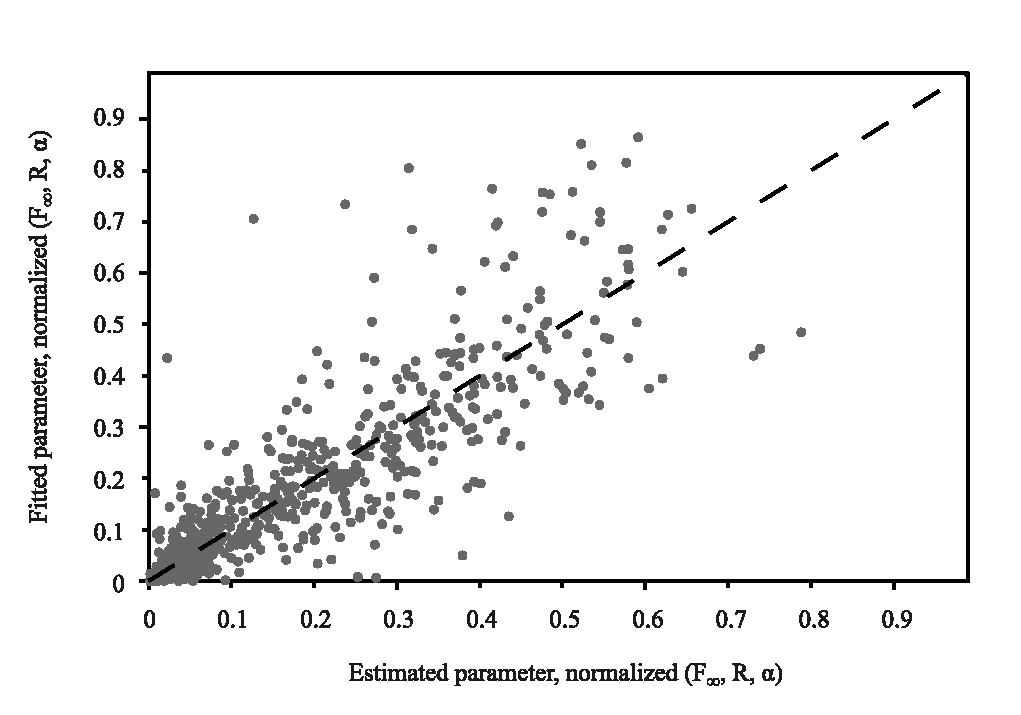
\includegraphics[width=\textwidth]{dpe_hyp.eps}
    \caption{Estimated regression parameters versus optimized regression 
    parameters (fitted after outliers were removed) for the hyperbolic model 
    (i.e., $F_{\infty}$, $R$, $\alpha$). Data is based on the monthly 
    partitioning of 25 flux towers during 2002. Parameter units have been 
    normalized for readability. The dashed line represents unity.}
    \label{fig:hmodest}
\end{figure}

Figure \ref{fig:hmodest} shows the relationship between the estimated parameters and optimized parameters for the hyperbolic model (i.e., equation \ref{eq:hypmod}).  
The units for each of three parameters have been normalized (i.e., values range between 0 and 1) for readability.  
The data is based on monthly regressions from 2002 of PPFD and NEE data pairs from 25 flux tower stations.  
A similar plot is shown in Figure \ref{fig:lmodest} where instead the regression parameters are shown for the linear model (i.e., equation \ref{eq:linmod}) for the same flux stations and time period.  
In both plots, the 1:1 line is shown for comparison.  
Both the hyperbolic and linear model parameter estimations exhibit moderately strong positively linear correlations to their optimized parameters ($r \approx 0.78$) suggesting that the dynamic parameterization methodology presented in equations \ref{eq:dpm1}--\ref{eq:dpm3} is suitable for this model.  
The simplicity of the dynamic parameterization model (requiring only mean, standard deviation, maximum and minimum of the observations) allows for the coefficients to be updated when new stations are included in the model.

%% ------------------------------------------------------------------------ %%
%% fig:lmodest | Linear model parameter estimates : optimized
%% ------------------------------------------------------------------------ %%
\begin{figure}[h!]
    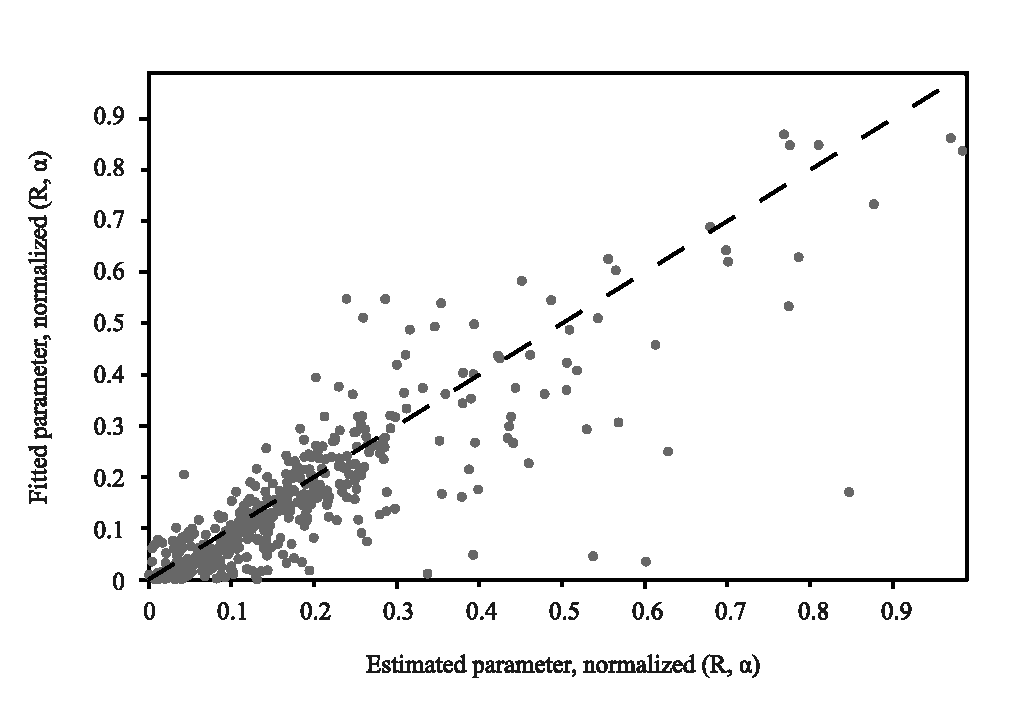
\includegraphics[width=\textwidth]{dpe_lin.eps}
    \caption{Estimated regression parameters versus optimized regression 
    parameters (fitted after outliers were removed) for the linear model 
    (i.e., $R$, $\alpha$). Data is based on the monthly partitioning of 25 flux 
    towers during 2002. Parameter units have been normalized for readability. 
    The dashed line represents unity.}
    \label{fig:lmodest}
\end{figure}

%% \\\\\\\\\\\\\\\\\\\\\\\\\\\\\\\\\\\\\\\\\\\\\\\\\\\\\\\\\\\\\\\\\\\\\\\\ %%
%% PART 3.2.5 -- STAGE 1: OUTLIER HANDLING
%% //////////////////////////////////////////////////////////////////////// %%
\subsection{Outlier handling}
\label{sec:mst1out}
The last data processing consideration is handling outliers.  
While there are morality debates over whether outliers should be removed at all from observation datasets, it is well known that outliers are detrimental when present during model fitting.  
This project is trying to address large scale processes and therefore removing outliers from instantaneous measurement fields to improve the fitted relationships between NEE and PPFD is viewed as acceptable.

To provide a robust and statistically-based approach for identifying outliers for stage 1 data pairs of NEE and PPFD, Peirce's criterion is used \parencite{peirce52}.  
The main issue revolving around Peirce's criterion is the calculation of the maximum allowable deviation of a measurement (i.e., the threshold error).  
To help facilitate this difficulty, tables of values were developed and published by B.A. Gould, Jr. \parencite{gould55}.  
Unfortunately, flux tower datasets often have numbers of observations that far exceed the values provided in Gould's tables. 
Therefore, in order to use Peirce's criterion, the error threshold values must be calculated.

The methodology follows Gould's algorithm and the calculation utilizes a Newtonian-style convergence method as presented by K. Thomsen\footnotemark. \footnotetext{http://mathforum.org/kb/thread.jspa?forumID=13\&threadID=1841790\\ \indent\&messageID=6449606} 
The principle of Peirce's criterion for identifying outliers is that \parencite{peirce52}:
\begin{quotation}
``the proposed observations should be rejected when the probability of the system of errors obtained by retaining them is less than that of the system of errors obtained by their rejection multiplied by the probability of making so many, and no more, abnormal observations.''
\end{quotation}

In this principle, Peirce proposes two systems, one where outliers have been identified and removed and the original system.  
To express this idea, the following condition for rejection is made \parencite[Eq. A]{gould55}:
%% ------------------------------------------------------------------------ %%
%% eq:goulda | Gould's equation A
%% ------------------------------------------------------------------------ %%
\nomenclature{$\lambda$}{Ratio of mean errors between Peirce's two systems}%
\nomenclature{$N$}{Total number of observations}%
\nomenclature{$n$}{Assumed number of outliers}%
\nomenclature{$x^{2}$}{Residual squared-error, (also Peirce's deviation)}%
\nomenclature{$\psi x$}{Probability of error exceedance}%
\nomenclature{$Q_{pc}$}{Peirce's condition for rejection}
\begin{equation}
\label{eq:goulda}
    \lambda^{N-n} e^{0.5\cdot n(x^{2}-1)}(\psi x)^{n} < Q_{pc}^{N}
\end{equation}

\noindent where: \\
\indent $\lambda$ = ratio of mean errors between the two systems \\
\indent $N$ = number of observations \\
\indent $n$ = number of outliers \\
\indent $x$ = residual error \\
\indent $\psi x$ = probability of error exceedance (hyperbolic base) \\
\indent $Q_{pc}$ = represents the condition for rejection, given by 
\parencite[Eq. B]{gould55}:
%% ------------------------------------------------------------------------ %%
%% eq:gouldb | Gould's equation B
%% ------------------------------------------------------------------------ %%
\begin{equation}
\label{eq:gouldb}
    Q_{pc}^{N} = \frac{n^{n}(N-n)^{N-n}}{N^{N}}
\end{equation}

Peirce proposes to begin with the assumption that the excess in the sum of the squared errors from the original system (compared to the system where outliers are removed) is equal to the sum of the squared errors of the outliers.  
This presents the following equation \parencite[Eq. C]{gould55}:
%% ------------------------------------------------------------------------ %%
%% eq:gouldc | Gould's equation C
%% ------------------------------------------------------------------------ %%
\nomenclature{$m$}{Number of model unknowns}
\begin{equation}
\label{eq:gouldc}
    x^{2} = 1 + \frac{N-m-n}{n}(1 - \lambda^{2})
\end{equation}

\noindent where: \\
\indent $x^{2}$ = Peirce's deviation (squared error threshold) \\
\indent $m$ = number of unknowns (fitting parameters) in the system \\

To solve this system of equations (i.e., determine the critical error, $x^{2}$, for which observations with a squared error less than this value should be kept and observations with a squared error greater than this value should be rejected), an iterative approach can be made by first allowing the following equality \parencite[Eq. D]{gould55}:
%% ------------------------------------------------------------------------ %%
%% eq:gouldd | Gould's equation D
%% ------------------------------------------------------------------------ %%
\nomenclature{$R_{pc}$}{In Peirce's criterion, $R_{pc} = e^{0.5(x^2-1)}\psi x$}
\begin{equation}
\label{eq:gouldd}
    R_{pc} = e^{0.5(x^2-1)}\psi x
\end{equation}

\noindent to be substituted into equation \ref{eq:goulda} to obtain the following \parencite[Eq. A$'$]{gould55}:
%% ------------------------------------------------------------------------ %%
%% eq:gouldap | Gould's equation A'
%% ------------------------------------------------------------------------ %%
\begin{equation}
\label{eq:gouldap}
    \lambda^{N-n} R_{pc}^{n} = Q_{pc}^{N}
\end{equation}

\noindent Now, for a given number of observations (i.e., $N$), an assumed number of outliers (i.e., $n$), and the number of fitting parameters used in the regression (i.e., $m$), the critical observation residual error (i.e., $x$) for identifying outliers can be calculated as follows:

\begin{enumerate}
    \item Calculate $Q_{pc}$ based on the N$^{th}$ root (equation \ref{eq:gouldb})
    \item Assume a starting value for $R_{pc}$ (e.g., 1.0)
    \item Calculate $\lambda$ based on the current $R$ value by taking the 
          1/(N-n)$^{th}$ root (equation \ref{eq:gouldap})
    \item Calculate $x^{2}$ based on the current $\lambda$ value (equation
          \ref{eq:gouldc})
    \item Calculate $R_{pc}$ based on the current $x^{2}$ value (equation 
          \ref{eq:gouldd})
    \item Compare the new $R_{pc}$ value to the one in step 3
    \item Repeat steps 3--6 until the difference between $R_{pc}$ values is 
          negligible 
\end{enumerate}

\noindent This algorithm can be expressed in the Python programming language by taking advantage of the third party modules NumPy\footnotemark \footnotetext{\url{http://www.numpy.org}} and SciPy\footnotemark. \footnotetext{\url{http://www.scipy.org}} 
An example of the code is given in Appendix \ref{app:peircepy}.

The following algorithm (example available in Appendix \ref{app:outlierpy}) can be used to make use of this code in identifying outliers in the GPP partitioning: 

\begin{enumerate}
    \item Fit a model (e.g., equation \ref{eq:linmod} or \ref{eq:hypmod}) to
          the observation data (i.e., NEE and PPFD pairs)
    \item Calculate the model's squared residual errors:\\
          %% ---------------------------------------------------------------%%
          %% eq:residerr | Residual error calculation
          %% ---------------------------------------------------------------%%
          \nomenclature{$U$}{Set of observations}%
          \nomenclature{$u$}{Set of model predictions of $U$}
          \begin{equation}
          \label{eq:residerr}
              x_{i}^{2} = (U_{i}-u_{i})^{2}
          \end{equation}
          where: $U_{i}$ = $i^{th}$ observation and $u_{i}$ = $i^{th}$ model 
          prediction
    \item Calculate the model mean squared error (MSE):\\
          %% ---------------------------------------------------------------%%
          %% eq:mse | Mean-squared error calculation
          %% ---------------------------------------------------------------%%
          \nomenclature{$\text{MSE}$}{Mean squared error}
          \begin{equation}
          \label{eq:mse}
              \text{MSE} = \frac{\sum_{i=1}^{N}(U_{i}-u_{i})^{2}}{N-m}
          \end{equation}
          where: $N$ is the number of observations and $m$ is the number of 
          regressors (i.e., model coefficients)
    \item Assume one outlier exists in the observation pairs (i.e., $n=1$)
    \item Calculate Peirce's $x^{2}$ using the Python script
    \item Calculate the maximum squared error deviation:\\
          %% ---------------------------------------------------------------%%
          %% eq:delta2 | Squared deviation (delta) calculation
          %% ---------------------------------------------------------------%%
          \nomenclature{$\Delta^{2}$}{Outlier threshold, squared-error}
          \begin{equation}
          \label{eq:delta2}
              \Delta^{2} = \text{MSE}\cdot x^{2}
          \end{equation}
    \item Identify any squared errors, $x_{i}^{2}$ (from step 2), greater than 
          $\Delta^{2}$
    \item Increment $n$ and repeat steps 5--7 until the number of outliers 
          found is less than $n$
\end{enumerate}

%% ------------------------------------------------------------------------ %%
%% fig:outlier | Peirce's criterion outlier identification/removal (red)
%% ------------------------------------------------------------------------ %%
\begin{figure}[h!]
    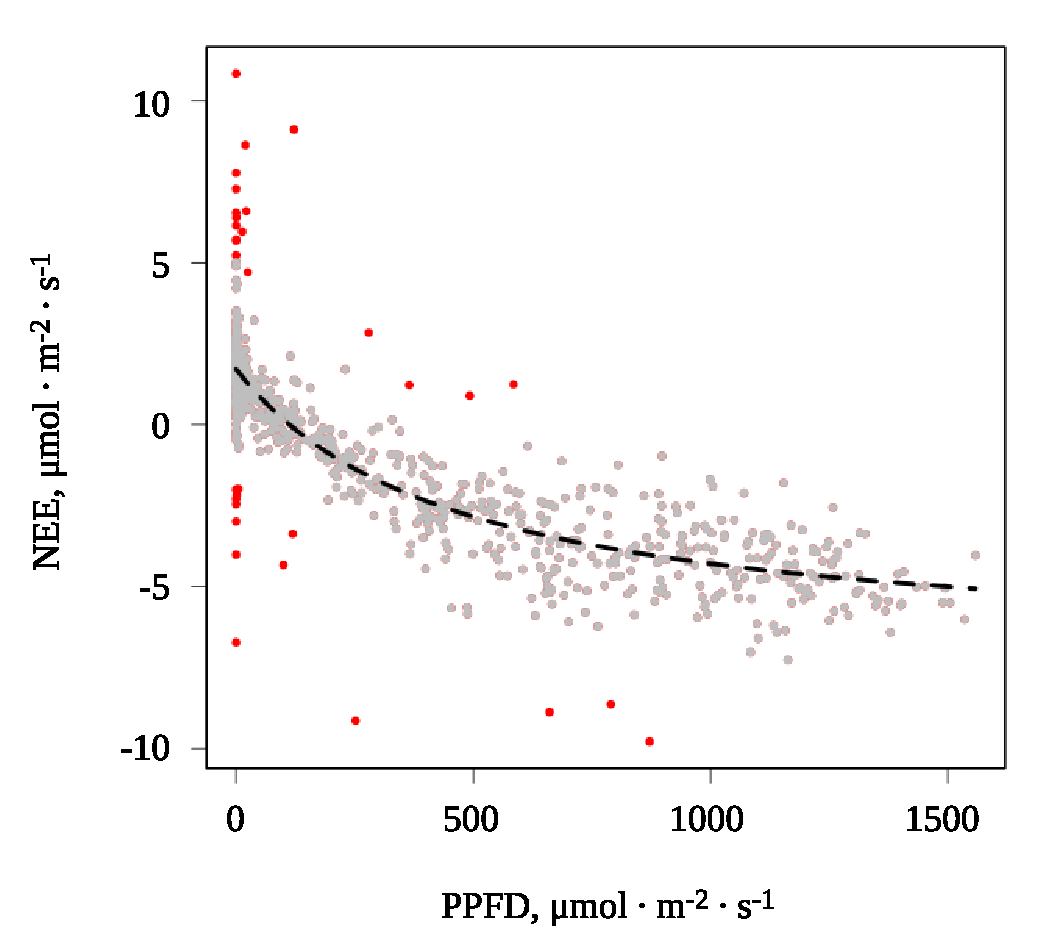
\includegraphics[width=0.85\textwidth]{olr_sedeg.eps}
    \caption{Plot of PPFD versus NEE for the month of August, 2004 for flux 
    tower SE-Deg (Sweden). Data points highlighted in red represent outliers 
    removed using the Peirce criterion. The dashed line represents the flux 
    partitioning as fitted by equation \ref{eq:hypmod}: $\alpha = 0.0189$, 
    $F_{\infty} = 8.8$, $R = 1.72$. The model fit coefficient of determination, 
    $R^{2}$, is 0.757 before outliers are removed and 0.872 after removal.}
    \label{fig:outlier}
\end{figure}

\noindent Figure \ref{fig:outlier} shows an example of the GPP partitioning for flux tower SE-Deg (located in Sweden) during May of 2002.  
Outliers identified by the Peirce criterion are highlighted in red ($N_{outliers} = 14$).  
Peirce's criterion successfully identifies observation pairs distant from the optimization curve (dashed line).  
Following the removal of the outliers, the partitioning regression fitness (based on equation \ref{eq:hypmod}) improves ($R^{2} = 0.796$ for the original observations; $R^{2} = 0.884$ after outliers are removed).  
In most cases, outliers are identified in a manner similar to that presented in Figure \ref{fig:outlier}.  
However, some cases have been noted when Peirce's criterion have identified observation pairs as outliers contrary to appearance.  
Based on 267 months of observation pairs (i.e., PPFD and NEE), the average percentage of outliers removed to observations is $\approx$2.4\% for the hyperbolic model (i.e., equation \ref{eq:hypmod}) and $\approx$5.6\% for the linear model (i.e., equation \ref{eq:linmod}).  
Overall, this method presents a sufficient and efficient identification and removal process for handling outliers. 
